\section{NGHIỆP VỤ}

Thông qua việc phân tích các yêu cầu của người dùng, nghiên cứu, ứng dụng các công nghệ hiện tại, đồng thời tham gia vào các chuyến du lịch Nhóm đã thống kê yêu cầu nghiệp vụ của ứng dụng và  xây dụng được một hệ thống thông tin Website du lịch như sau: 
\\
\\
\textbf{Bộ phận người dùng: } 
\begin{itemize}
    \item Người dùng không có tài khoản 
    \item Người dùng có tài khoản
\end{itemize}
\textbf{Người dùng không có tài khoản: }
Người dùng không có tài khoản chỉ sử dụng được một số chức năng cơ bản của hệ thống như : 
\begin{itemize}
    \item Xem thông tin kế hoạch du lịch có sẵn.
    \item Xem thông tin các tour du lịch.
    \item Xem thông tin các bài review, gợi ý địa điểm du lịch ở nơi họ muốn tới.
\end{itemize}
\textbf{Người dùng có tài khoản:} Sử dụng được tất cả chức năng của hệ thống và chính là nhóm đối tượng đề tài hướng tới. Để sỡ hữu tài khoản cho riêng cho cá nhân cũng như những trải nghiệm tốt nhất với hệ thống thì có một số quy trình chính như: 
\begin{quote}
    \textbf{Quy trình người dùng đăng kí tài khoản hệ thống: }
    \begin{itemize}
        \item Người dùng vào trang đăng kí tài khoản.
        \item Người dùng đăng ký tài khoản thông qua email.
        \item Thông tin tài khoản bao gồm email, username, họ và tên, ngày sinh, số điện thoại,.... trong đó thông tin họ và tên, email là bắt buộc.
    \end{itemize}
    \textbf{Quy trình người dùng đăng nhập vào hệ thống: }
    \begin{itemize}
        \item Người dùng vào trang đăng nhập và đăng nhập bằng tài khoản và mật khẩu đã đăng kí.
        \item Người dùng có thể đăng nhập thông qua googleID (gmail)
    \end{itemize}
    \textbf{Quy trình tạo kế hoạch cho chuyến đi: }
    \begin{itemize}
        \item Sau khi tham khảo các vài review cũng như các kế hoạch có sẵn thì người dùng có thể tiến hành tạo kế hoạch của mình.
        \item Người dùng chọn ngày khởi hành và khứ hồi.
        \item Người dùng chọn địa điểm đến.  
        \item Người dùng chọn chế độ cho kế hoạch "Private" và "Public".
        \item Người dùng nhấn "Khởi tạo" để chuyển sang giao diện thêm chi tiết hoạt động mỗi ngày cho chuyến đi.
        \item Người dùng chọn mốc thời gian cho các hoạt động của chuyến đi.
        \item Người dùng chọn khách sạn dừng chân cho chuyến đi, sau khi chọn type là "Hotel" thì sẽ có giao diện googlemap hiển thị các khách sạn nổi tiếng cũng như có lượt vote cao gợi ý cho khu vực người dùng muốn đến.
        \item Người dùng chọn địa điểm ăn uống, sau khi chọn type là "Eat n Drink" thì sẽ có giao diện googlemap hiển thị tất cả các quán ăn, các tiệm nước nổi bật cũng như có lượt vote cao trong khu vực đã chọn.
        \item Người dụng chọn các địa điểm du lịch thu thu hút đông khách du lịch ở địa phương thông qua type "Attraction".
        \item Sau khi đã chọn xong thì ngừời dùng nhấn "Add" để thêm các hoạt động chi tiết trong một ngày vào kế hoạch.
        
    \end{itemize}
     \textbf{Quy trình tạo bài review giới thiệu địa điểm du lịch:  }
     \begin{itemize}
         \item Sau khi đã trải nghiệm xong chuyến du lịch người dùng có thể viết bài review cho địa điểm mà mình đã đi.
         \item Người dùng chọn tạo bài blog.
         \item Người dùng chọn địa điểm đã đi 
         \item Người dụng chọn mốc thời gian đã đi
         \item Người dùng viết một bài blog cho những trải nghiệm thực của mình kèm thêm thông tin hình ảnh.
         \item Người dùng nhấn "Create" để bài blog cho mình.
         
     \end{itemize}
     \textbf{Quy trình người dùng gởi lời mời kết bạn: }
     \begin{itemize}
         \item Mỗi tài khoản người dùng có thể kết bạn và tương tác với nhiều người dùng khác.
         \item Người dùng nhấn "Friend" hoặc nhập tên người mình muốn kết bạn ở ô "Search" để xuất hiện giao điện những người mà mình muốn kết bạn.
         \item Người dùng nhấn "Add Friend" để gởi lời mời kết bạn đến đối phương.
         \item Người dùng nhấn "Delete" để xoá thông tin không phải người mình muốn kết bạn.
         
     \end{itemize}
     \textbf{Quy trình người dùng tương tác với lời mời kết bạn:  }
     \begin{itemize}
         \item Người dùng nhấn vào "Friend" để xem thông tin lời mời kết bạn mà các người dùng khác đã gởi cho mình.
        \item Người dùng nhấn "Accecpt" để đồng ý lời mời kết bạn.
        \item Người dùng nhấn "Decline" để từ chối lời mời kết bạn.
     \end{itemize}
     \textbf{Quy trình người dùng trò chuyện với nhau: }
     \begin{itemize}
         \item Người dùng nhấn vào "Messenger" hoặc biểu tượng Chat để mở giao diện trò chuyện.
         \item Người dùng chỉ có thể trò chuyện với bạn của mình.
         \item Người dùng có thể kiểm tra xem bạn bè có đang cùng hiện hữu không thông qua chấm xanh và đỏ ở góc hình avatar đối phương.
         \item Tại giao diện người dùng chọn người mình muốn trò chuyện, gõ thông tin cần nói là nhấn "Send". 
     \end{itemize}
     \textbf{Quy trình người dùng xem và tương các bài blog review: }
    \begin{itemize}
        \item Người dùng nhấn vào danh sách các bài Blog để xem danh sách các bài chú ý.
        \item Người dùng nhấn vào bài cần đọc.
        \item Tại giao diện blog người dùng có thể tương tác bằng cách thả like hoặc comment nhận xét.
    \end{itemize}
    \textbf{Quy trình người dùng xem các kế hoạch có sẵn: }
    \begin{itemize}
        \item Người dùng nhấn vào danh sách các kế hoạch có sẵn.
        \item Người dùng nhập vào ô tìm kiếm địa điểm mình muốn tham khảo và nhấn "Search".
        \item Giao diện sẽ xuất hiện tất cả các kế hoạch có sẵn về địa điểm mà người dùng muốn tìm kiếm.
        \item Người dùng chọn cho mình kế hoạch muốn xem.
    \end{itemize}
    
    \textbf{Quy trình người dùng chia sẻ kế hoạch của mình cho bạn bè: }
    \begin{itemize}
        \item Người dùng nhấn vào biểu tượng chia sẻ trên kế hoạch của mình.
        \item Hiển thị danh sách bạn bè muốn chia sẻ.
        \item Chọn bạn bè muốn chia sẻ và nhấn "Share"
        \item Hiển thị thông báo thành công.
    \end{itemize}
\end{quote}

   




\section{Mô hình phát triển website - Model View Controller}
\subsection{Mô hình phát triển website}
Kiến trúc Model-View-Controller (MVC) chia ứng dụng thành nhóm của ba thành phần chính: Models, Views, Controllers. Khi sử dụng khung mẫu lập trình này, yêu cầu (request) được chuyển cho Controller, Controller có trách nhiệm làm việc với Model để thực hiện yêu cầu của người dùng hoặc lấy dữ liệu từ cơ sở dữ liệu. Controller lựa chọn View để hiển thị ra với người dùng, cung cấp cho View những dữ liệu lấy từ Model.
Hình \ref{fig:mvcmodel} thể hiện những tương tác, truy vấn dữ liệu ở mỗi thành phần trong mô hình MVC, Controller sử dụng thông tin từ yêu cầu của người dùng để đưa ra những truy vấn dữ liệu thích hợp cho Model, từ đó dữ liệu được ghép chung với View để chuyển tới người dùng.
\begin{itemize}
    \item Model trong ứng dụng MVC thể hiện trạng thái của ứng dụng và các business rule. Các dữ liệu của công ty nên được tạo, lưu trữ, thay đổi dựa trên Model, dựa trên việc hiện thực tương tác, ràng buộc dữ liệu hợp lý để bảo đảm sự ổn định của ứng dụng.
    \item View có nhiệm vụ biểu diễn nội dung thông qua giao diện người dùng. Có thể nhúng trực tiếp dữ liệu vào HTML.
    \item Controller đóng vai trò trung gian giữa Model và View. Xử lí các yêu cầu của người dùng. Làm việc với Model và lựa chọn View để thể hiện nội dung một cách thích hợp.
\end{itemize}

Trong mô hình MVC, View chỉ hiển thị thông tin, Controller nhận, xử lý, phản hồi các yêu cầu, tương tác của người dùng. Controller là điểm khởi đầu, có trách nhiệm lựa chọn Model cần làm việc cùng, View cần để tạo nội dung.
\begin{figure}[H]
\centering
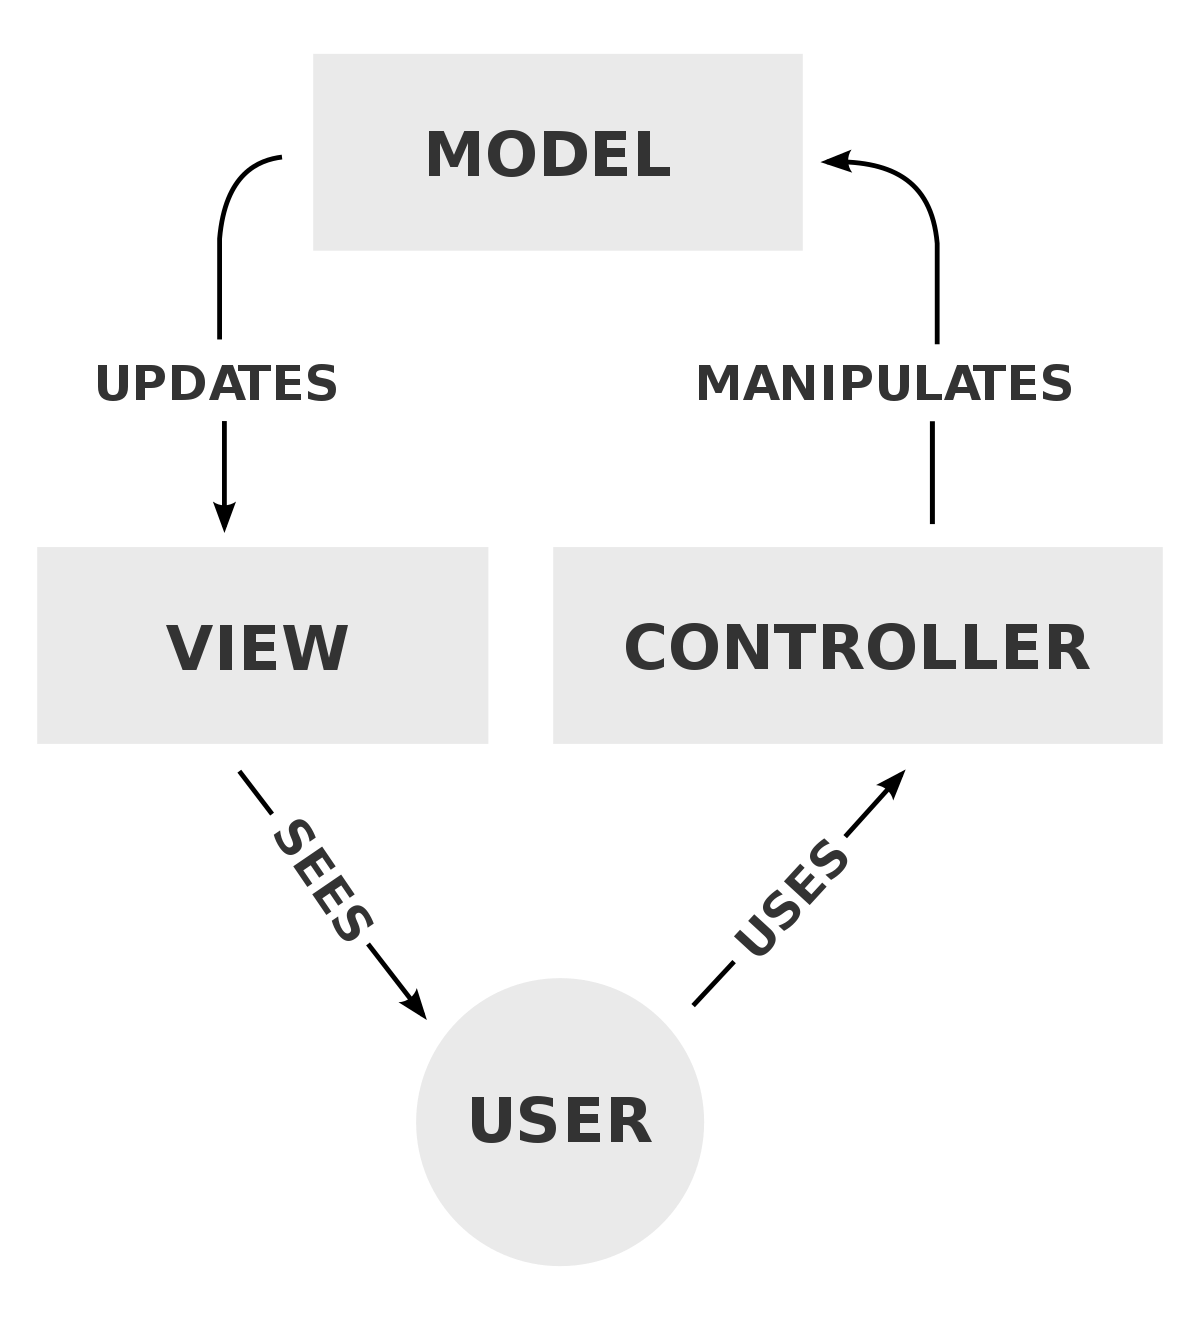
\includegraphics[width=10cm]{image/MVC.png}
\caption{Mô hình MVC}
\label{fig:mvcmodel}
\end{figure}

\section{Ứng dụng đa trang và ứng dụng đơn trang}
\subsection{Ứng dụng đa trang - Multi page application}
Ứng dụng đa trang hoạt động theo cách cơ bản nhất. Mọi thay đổi khi lấy dữ liệu, gửi dữ liệu lên máy chủ đều yêu cầu cập nhật lại toàn bộ trang bằng dữ liệu mới được gửi từ máy chủ, và hiện lên trình duyệt. Những trang này thường có kích thước lớn. Nhờ có AJAX, các ứng dụng đa trang hiện nay không cần truyền nhiều dữ liệu từ máy chủ đến trình duyệt. Chỉ cần làm mới những phần đi kèm với dữ liệu được thay đổi. Tuy nhiên, việc này trở nên phức tạp khi ứng dụng càng lớn.

Ưu điểm: 
\begin{itemize}
    \item Người dùng dể dàng thao tác trên ứng dụng cho các menu, điều hướng ít.
    \item Ứng dụng tốt các kỹ thuật SEO. Do ứng dụng chia thành nhiều trang, nên có thể tối ưu từng từ khóa cho mỗi trang.
\end{itemize}

Nhược điểm: 
\begin{itemize}
    \item Quá trình phát triển thường yêu cầu sự kết hợp chặt chẽ ở backend và frontend trong quá trình xử lý, nhận dữ liệu.
    \item Thời gian phát triển thường lớn khi so sánh với ứng dụng đơn trang.
\end{itemize}
\subsection{Ứng dụng đơn trang - Single page application}
Ứng dụng đơn trang tương tự như một ứng dụng ở trong trình duyệt, không yêu cầu quá trình tải lại trang khi sử dụng, nên giảm được thời gian chờ. Người dùng chỉ cần tải trang lần đầu, sau đó các nội dung sẽ được tải xuống bằng cách sử dụng JavaSript.
Ứng dụng đơn trang thường tách biệt giữa dữ liệu và HTML, CSS, trình duyệt sẽ trực tiếp hỗ trợ việc tạo nội dung. 


Ưu điểm: 
\begin{itemize}
    \item SPA nhanh, do hầu hết các tài nguyên (HTML, CSS, Scripts) được tải một lần trong suốt quá trình sử dụng ứng dụng. Chỉ có dữ liệu được truyền qua lại giữa trình duyệt và máy chủ.
    \item Quá trình phát triển thường đơn giản hơn. Do khi phát triển, lập trình viên không cần quan tâm đến việc tạo toàn bộ trang web ở phía máy chủ.
    \item SPA dễ dàng kiểm tra, kiểm lỗi hơn do phần lớn các trình duyệt (Chrome, FireFox,...) hỗ trợ tốt trong việc quan sát, debug, kiểm lỗi ngay trên trình duyệt.
    \item SPA có khả năng làm việc với bộ nhớ cục bộ, cache tốt. Nên hiệu quả hơn ứng dụng đa trang khi làm việc offline, do các tài nguyên chỉ cần tải xuống một lần.
\end{itemize}
Nhược điểm: 
\begin{itemize}
    \item Tải xuống thường lâu ở thời điểm đầu do lượng lớn tài nguyên cần tải xuống ở phía người dùng.
    \item JavaScript cần được cho phép chạy ở phía người dùng.
    \item Thường ít bảo mật hơn khi so sánh ứng dụng đa trang do XSS (Cross Site Scripting), cho phép kẻ tấn công có thể chèn mã phá hoại vào ứng dụng web tới người dùng khác.
    \item Rõ rỉ bộ nhớ có thể làm cho máy tính người dùng bị chậm đi đáng kể.
\end{itemize}

\subsection{Kết luận và lựa chọn}
Do khối lượng công việc, cũng như tính năng mà hệ thống ở luận văn cung cấp cho người dùng. Việc sử dụng SPA, ứng dụng đơn trang tỏ ra hiệu quả hơn. 
\begin{itemize}
    \item Việc chia nhỏ hệ thống ra thành nhiều phần nhỏ, quản lý, hiện thực ở SPA đơn giản hơn MPA.
    \item Hệ thống cần lưu trữ, chia sẽ nhiều dữ liệu giữa các tính năng, tác vụ. Do đó với SPA, có thể tận dụng bộ nhớ cục bộ (local storage) để hỗ trợ việc tương tác với người dùng.
    \item SPA đang được sử dụng rất nhiều, do đó có nhiều framework hỗ trợ, cộng đồng phát triển.
    \item Hệ thống được phát triển hỗ trợ cho hoạt động của đoàn khoa, do đó không cần chú trọng vào quản lý SEO.
\end{itemize}
Từ một số đặc điểm kể trên, nhóm quyết định lựa chọn mô hình ứng dụng đơn trang kết hợp với Model - View - Controller để phát triển hệ thống.
\section{Các nền tảng cho Javascript}
Khi lựa chọn xây dựng ứng dụng đa trang, có rất nhiều nền tảng, công nghệ hiện thực trên JavaScript hỗ trợ cho việc xây giao diện người dùng (front-end). Nâng cao hiệu suất công việc cũng như hỗ trợ quản lí mã nguồn tốt, ví dụ như Angular, ReactJS, VueJS. Sau đây nhóm sẽ giới thiệu, phân tích ưu nhược điểm một số công nghệ và đưa ra lựa chọn.

\subsection{AngularJs}
Angular là một framework được viết bằng TypeScript. Được phát triển bởi Google và được sử dụng trong Google AdWords, một dự án quan trọng của Google. Angular có cấu trúc cho các ứng dụng web động. Nó cho phép sử dụng HTML như là ngôn ngữ mẫu và cho phép mở rộng cú pháp của HTML để diễn đạt các thành phần ứng dụng một cách rõ ràng và súc tích. Hai tính năng cốt lõi: Data binding và Dependency injection của AngularJS loại bỏ phần lớn code thường phải viết. Nó xảy ra trong tất cả các trình duyệt, làm cho nó trở thành đối tác lý tưởng của bất kỳ công nghệ Server nào.
\subsection{VueJS}

\textbf{Vue.js} là một framework linh động (nguyên bản tiếng Anh: progressive – tiệm tiến) dùng để xây dựng giao diện người dùng (user interfaces). Khác với các framework nguyên khối (monolithic), VueJS được thiết kế từ đầu theo hướng cho phép và khuyến khích việc phát triển ứng dụng theo từng bước. Khi phát triển lớp giao diện (view layer), người dùng chỉ cần dùng thư viện lõi (core library) của VueJS, vốn rất dễ học và tích hợp với các thư viện hoặc dự án có sẵn. Cùng lúc đó, nếu kết hợp với những kĩ thuật hiện đại như SFC (single file components) và các thư viện hỗ trợ, VueJS cũng đáp ứng được dễ dàng nhu cầu xây dựng những ứng dụng một trang (SPA - Single-Page Applications) với độ phức tạp cao hơn nhiều.

\subsection{ReactJS}

\textbf{ReactJs} là một thư viện Javascript đang nổi lên trong những năm gần đây với xu hướng Single Page Application. Trong khi những framework khác cố gắng hướng đến một mô hình MVC hoàn thiện thì React nổi bật với sự đơn giản và dễ dàng phối hợp với những thư viện Javascript khác. Nếu như AngularJS là một Framework cho phép nhúng code Javascript trong code HTML thông qua các thược tính như ng-model, ng-repeat...thì với ReactJS là một thư viện cho phép nhúng code HTML trong code Javascript nhờ vào JSX, điều đó giúp dễ dàng lồng các đoạn HTML vào trong JS. Tích hợp giữa Javascript và HTML vào trong JSX làm cho các component dễ hiểu hơn. Một trong những điểm hấp dẫn của React là thư viện này không chỉ hoạt động trên phía client, mà còn được render trên server và có thể kết nối với nhau. React so sánh sự thay đổi giữa các giá trị của lần render này với lần render trước và cập nhật ít thay đổi nhất trên DOM. Nhờ đó ReactJS có hiệu năng tốt hơn những công nghệ hiện tại.

\subsection{Kết luận và lựa chọn}
Như đã đề cập ở trên, ReactJs là một Thư viện Javascript được tạo ra bởi sự cộng tác giữa Facebook và Instagram. Việc lựa chọn ReactJs là công cụ phát triển được dựa trên nhiều tiêu chí bao gồm hướng tiếp cận, trải nghiệm người dùng, thư viện hỗ trợ từ cộng đồng,... Điểm qua vài ưu điểm của ReactJs như sau:
\begin{itemize}
    \item ReactJS tạo ra cho chính nó DOM ảo – nơi mà các component thực sự tồn tại trên đó. Điều này sẽ giúp cải thiện hiệu suất rất nhiều. ReactJS cũng tính toán những thay đổi nào cần cập nhật lên DOM và chỉ thực hiện chúng. Điều này giúp ReactJS tránh những thao tác cần trên DOM mà nhiều chi phí.
    \item ReactJS giúp việc viết các đoạn code JS dễ dàng hơn: Nó dùng cú pháp đặc biệt là JSX (Javascript mở rộng) cho phép ta trộn giữa code HTML và Javascript. Ta có thể thêm vào các đoạn HTML vào trong hàm render mà không cần phải nối chuỗi. Đây là đặc tính thú vị của ReactJS. Nó sẽ chuyển đổi các đoạn HTML thành các hàm khởi tạo đối tượng HTML bằng bộ biến đổi JSX.
    \item Một trong những vấn đề với các ứng dụng đơn trang là tối ưu SEO và thời gian tải trang. Nếu tất cả việc xây dựng và hiển thị trang đều thực hiện ở client, thì người dùng sẽ phải chờ cho trang được khởi tạo và hiển thị lên. Điều này thực tế là chậm. Hoặc nếu giả sử người dùng vô hiệu hóa Javascript thì sao? ReactJS là một thư viện component, nó có thể vừa render ở ngoài trình duyệt sử dụng DOM và cũng có thể render bằng các chuỗi HTML mà server trả về. 
    \item Hiệu năng cao đối với các ứng dụng có dữ liệu thay đổi liên tục, dễ dàng cho bảo trì và sửa lỗi.
\end{itemize}

\section{Các thư viện cho ReactJS}
\subsection{Flux}
Flux là một kiến trúc mà Facebook sử dụng trong khi làm việc với React. Flux không phải là một \textbf{framework} hay một \textbf{thư viện (library)}. Nó đơn giản chỉ là một kiểu kiến trúc mới hỗ trợ thêm cho React, đồng thời xây dựng ý tưởng về luồng dữ liệu một chiều \textbf{(Unidirectional Data Flow)}.

\textbf{Cấu trúc của Flux:}
\begin{itemize}
    \item \textbf{Actions} - Làm nhiệm vụ truyền dẫn dữ liệu tới Dispatcher (được coi như các Helper Method)
    \item \textbf{Dispatcher} - Nhận thông tin từ Actions, truyền tải dữ liệu \textbf{(payload)} tới các nơi đã đăng ký nhận thông tin.
    \item \textbf{Stores} - Là nơi lưu trữ trạng thái và các logic của hệ thống, đây chính là nơi sẽ đăng ký nhận dữ liệu với Dispatcher.
    \item \textbf{Controller Views} - Chính là các React Components, làm nhiệm vụ nhận các trạng thái \textbf{(state)} từ \textbf{Stores} và truyền dữ liệu (dưới dạng \textbf{props}) cho các thành phần con.
\end{itemize}
\textbf{Mô hình hoạt động:}


\begin{figure}[H]
\centering
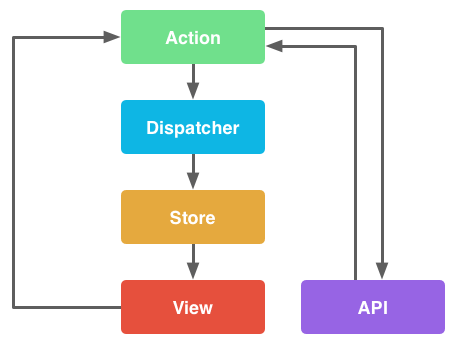
\includegraphics[width=10cm]{image/Redux-work-model.png}
\caption{Sơ đồ chung về quan hệ giữa các thành phần trong Flux}
\label{fig:redux_model}
\end{figure}
\textbf{Giải thích các thành phần trong hình \ref{fig:redux_model}:}
\begin{itemize}
    \item \textbf{Views} chính là thành phần làm nhiệm vụ hiển thị nội dung ứng dụng (thành phần này có nét tương đồng như thành phần \textbf{View} trong mô hình \textbf{MVC}).
    \item Khi người dùng tương tác với ứng dụng làm thay đổi trạng thái \textbf{(state)} của ứng dụng (Ví dụ như là các thao tác cơ bản trên dữ liệu: thêm, sửa, xóa), \textbf{View} sẽ thông qua \textbf{Action} gửi các thông tin thay đổi tới \textbf{Dispatcher} bao gồm:
    \begin{itemize}
        \item \textbf{action\_name}: tên của \textbf{Action} (Ví dụ: ADD\_USER).
        \item \textbf{action\_payload}: Nội dung muốn gửi (Ví dụ: firstname, lastname, email).
    \end{itemize}
    \item Sau khi nhận được thông tin từ \textbf{Action}, \textbf{Dispatcher} làm nhiệm vụ truyền tải \textbf{(broadcast)} nội dung nhận được tới các \textbf{Store} đăng ký lắng nghe sự kiện thay đổi từ trước đó.
    \item \textbf{Store} sau khi nhận thông tin, nó sẽ tiến hành việc cập nhật dữ liệu (Việc cập nhật dữ liệu này giống việc \textbf{setState} của Component).
    \item Sau khi cập nhật, \textbf{Store} bắn sự kiện xuống \textbf{View} để tiến hành cập nhật hiển thị cho người dùng.
    \item \textbf{API} giúp đỡ việc lấy dữ liệu từ Remote Server.
\end{itemize}


Sơ đồ trên đảm bảo luồng dữ liệu di chuyển trong Flux bắt buộc đi theo một đường nhất định.
\subsection{Redux}
Redux là một công cụ quản lý các trạng thái dự đoán được \textbf{(predictable state management tool)} cho các ứng dụng \textbf{Javascript}. Redux giúp bạn viết các ứng dụng hoạt động một cách nhất quán, chạy trong các môi trường khác nhau (client, server, và native) và dễ dàng kiểm thử.


\textbf{Cách thức Redux hỗ trợ ReactJS}


ReactJS được xây dựng theo một cách sao cho các \textbf{Components} đến việc quản lý nội bộ các \textbf{state} của chúng mà không cần bất kỳ một thư viện nào từ bên ngoài. ReactJS sẽ hoạt động tốt với các ứng dụng có ít component, nhưng khi ứng dụng trở lên lớn hơn thì việc quản lý các state được chia sẻ qua các component sẽ biến thành các công việc phức tạp.


Trong ReactJS, để truyền dữ liệu thông qua các \textbf{Component}, phải đảm bảo state luôn sống trong component cha, một \textbf{method} để cập nhật state trong chính component cha này và truyền cả state và method dưới dạng \textbf{props} đến các component con. Đây mới chỉ là cách thức truyền state trong các component cha - con, việc truyền state giữa các component có quan hệ cách xa nhau thì đó là một vấn đề lớn. Điều này khiến cho bộ phận quản lý state trong ứng dụng trở nên vô cùng phức tạp và Redux đã giải quyết được vấn đề đó.


\textbf{Cách thức hoạt động của Redux:}

Redux có \textbf{store} để lưu trữ toàn bộ \textbf{state} của ứng dụng. Bất kỳ component nào cũng có thể truy cập trực tiếp đến state được lưu trữ thay vì phải truyền theo \textbf{props} từ component này đến component khác! Redux có 3 thành phần chính: \textbf{Actions, Store, Reducers}
\begin{enumerate}
    \item \textbf{Actions}
    \begin{itemize}
        \item \textbf{Actions} đơn giản là các sự kiện, là cách thức gửi dữ liệu từ ứng dụng đến \textbf{store}. Những dữ liệu này có được từ sự tương tác của người dùng với ứng dụng, các lệnh gọi API hoặc từ các biểu mẫu \textbf{(form)}.
        \item \textbf{Actions} được gửi bằng cách sử dụng phương thức \textbf{store.dispatch()}. Các Actions phải có một thuộc tính \textbf{type} để diễn tả loại action, chúng cũng phải có một \textbf{payload} để chứa thông tin. Ví dụ như hình \ref{fig:redux-action-creator}
        \begin{figure}[H]
            \centering
            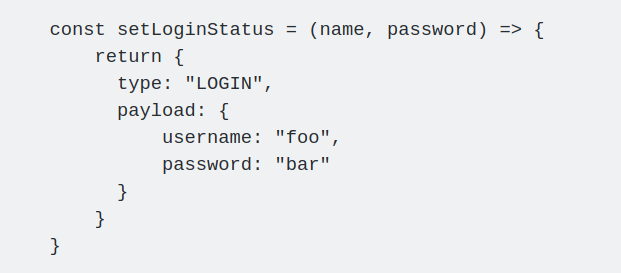
\includegraphics[width=10cm]{image/redux-action-creator.png}
            \caption{Một Action creator}
            \label{fig:redux-action-creator}
        \end{figure}
    \end{itemize}
    \item \textbf{Reducers}
    \begin{itemize}
        \item \textbf{Reducers} là các \textbf{hàm nguyên thủy}. Reducers lấy state hiện tại của ứng dụng, thực hiện một \textbf{action} và trả về một state mới. Những state này được lưu như những \textbf{Objects} và chúng định rõ cách state của một ứng dụng thay đổi trong việc phản hồi một action được gửi đến store.
    \end{itemize}
    \item \textbf{Store}
    \begin{itemize}
        \item \textbf{Store} lưu các \textbf{state} của ứng dụng và nó là \textbf{duy nhất} trong bất kỳ một ứng dụng Redux nào. Bạn có thể truy cập, cập nhật các state này.
        \item \textbf{Actions} thực hiện trên một state luôn luôn trả về một state mới. Vì vậy, state này là đơn giản và dễ đoán.
    \end{itemize}
\end{enumerate}


\subsection{Kết luận và lựa chọn}
\textbf{Flux} và \textbf{Redux} là 2 cái tên không xa lạ gì với cộng đồng \textbf{ReactJS}, chúng được sử dụng trong hầu hết các ứng dụng Javascript.


Kiến trúc của Flux tập trung giải quyết \textbf{'state changing'} rất hiệu quả. Tuy nhiên, Flux chỉ được Facebook giới thiệu như là một kiến trúc tổng quát ngoài ra họ không cung cấp cách hiện thực chi tiết nên ở ngoài cộng đồng hiện đã có rất nhiều phiên bản hiện thực lại, nổi tiếng nhất trong đó chính là Redux.


Điều làm cho Redux trở nên đặc biệt đó là REDUCER không bao giờ thay đổi state hiện tại của ứng dụng. Thay vào đó nó sẽ sao chép và trả về một state mới. Hướng tiếp cận này thường được thấy trong các ngôn ngữ hiện đại và thường được gọi là "state bất biến" \textbf{(“Immutable state”)}.


Tóm lại Flux và Redux là kiến trúc để quản lý state trong ứng dụng hiệu quả hơn. Flux là ý tưởng, kiến trúc tổng quát còn Redux là phiên bản được hiện thực lên từ Flux nên sẽ chi tiết hơn và sử dụng "immutable state" thay vì "mutable state". Chính vì điều này nên chúng ta sẽ thấy Redux khá phổ biến hơn là Flux và Redux sẽ thích hợp hơn với đề tài của nhóm.
\section{Bộ tiền xử lý}
\subsection{LESS}
LESS giúp viết các đoạn mã CSS đơn giản, ngắn gọn và hiệu quả hơn, đồng thời cũng dễ quản lý hơn bằng cách thêm vào CSS các thành phần động như biến, mixins, toán tử và hàm. LESS được phát triển bởi một lập trình viên người Đức là Alexis Sellier. Các thành phần cơ bản của LESS:
\begin{itemize}
	\item Biến được khai báo và sử dụng gán giá trị cho các thuôc tính. Ví dụ biến @color được sử dụng cho thuộc tính background-color trong class1
	\begin{verbatim}
	@color: #2d5e8b;
		.class1 {
		background-color: @color;
	}
	\end{verbatim}
	\item Mixins cho phép gắn toàn bộ thuộc tính của một class trong CSS vào trong class khác bằng cách thêm tên class này như một thuộc tính của class kia. Nó gần giống với biến, nhưng thay giá trị bằng toàn bộ các thuộc tính của class. Mixins cũng có thể được sử dụng như hàm, bằng cách truyền tham số.
	\begin{verbatim}
	.bordered {
		border-top: dotted 1px black;
		border-bottom: solid 2px black;
	}
	#menu a {
		color: #111;
		.bordered;
	}
	\end{verbatim}
\end{itemize}

\subsection{SASS}
    \begin{figure}[H]
        \centering
        
\includegraphics[width = 7cm]{image/sass-logo.png}
        \caption{SASS (Syntactically Awesome StyleSheets)}
        \label{fig:sass_logo}
    \end{figure}
    SASS (Syntactically Awesome StyleSheets) là một phần mở rộng của CSS, nó giúp chúng ta sử dụng biến (variables), quy tắc xếp chồng (nested rules), mixins, thừa kế (selector inheritance), hàm (functions), ... và hoàn toàn tương thích với cú pháp của CSS.
    
\subsection{Các đặc tính của SASS}
    \begin{itemize}
        \item Hoàn toàn tương thích với CSS.
        \item Mở rộng ngôn ngữ như các biến (variable), mixins, hàm (function), ...
        \item Nhiều function hữu ích cho các thao tác với màu sắc và các giá trị khác.
        \item Các đặc tính nâng cao như các control directive.
        \item Có cấu trúc, tùy biến đầu ra. SASS có hai định dạng file là *.sass và *.scss. Và cách viết của hai định dạng này cũng là khác nhau (nhưng các control directive, function thì có cùng một ý nghĩa).
    \end{itemize}
\subsection{@-Rules và Directives}
    \begin{itemize}
        \item @import\\
        Cho phép import các rule, style, biến, mixins, functions, ... từ một file SASS khác. Và nó sẽ được gộp lại thành một file khi xuất ra file CSS. Directive @import nhận một chuỗi là tên file sẽ được import. Mặc định, khi tên file không có phần mở rộng (extension), thì nó sẽ ưu tiên tìm file có phần mở rộng là *.scss và *.sass
        \begin{figure}[H]
            \centering
            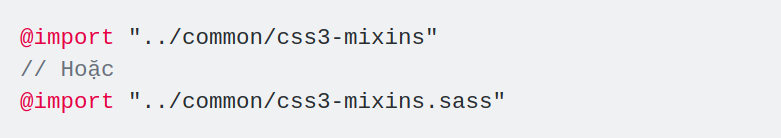
\includegraphics[width = 10cm]{image/sass-import.png}
            \caption{Ví dụ về @import}
            \label{fig:sass_import}
        \end{figure}
        \item @extend\\
        Cho phép bạn thừa kế các property của một class khác.
        \begin{figure}[H]
            \centering
            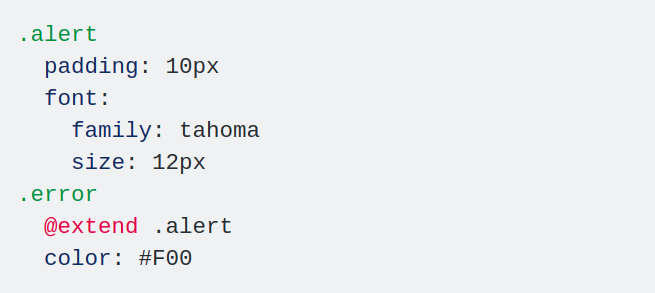
\includegraphics[width = 10cm]{image/sass-extend.png}
            \caption{Ví dụ về @extend}
            \label{fig:sass_extend}
        \end{figure}
        \item @each\\
        Giúp bạn duyệt một danh sách các giá trị, được dùng trong trường hợp phải viết một số lệnh giống nhau, nhưng chỉ khác chút về giá trị của thuộc tính.
        \begin{figure}[H]
            \centering
            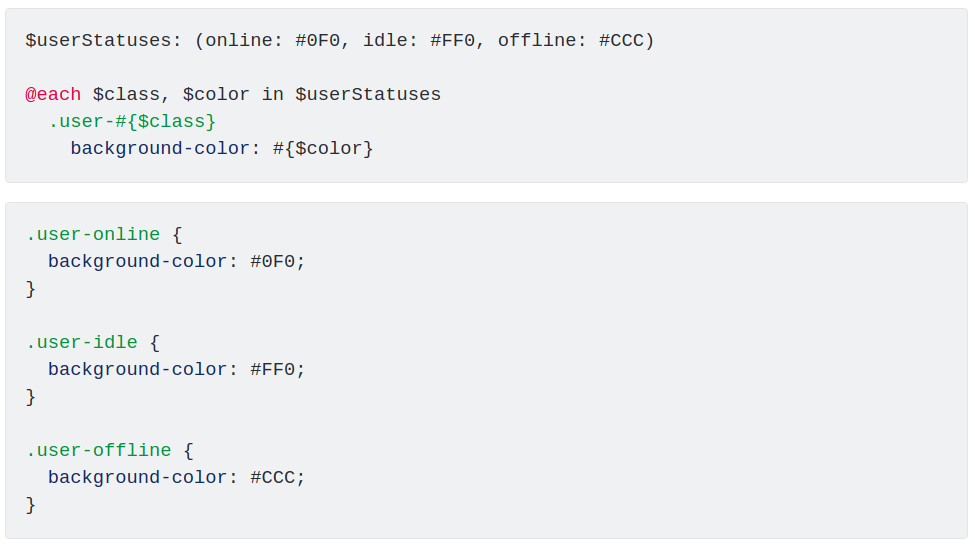
\includegraphics[width = 0.9\linewidth]{image/sass-each.png}
            \caption{Ví dụ về @each}
            \label{fig:sass_each}
        \end{figure}
        \item @mixin\\
        Giúp bạn định nghĩa một khối các style có thể được sử dụng lại nhiều lần. Trong SASS, ngoài @mixin còn @function, về bản chất nó giống nhau. Nhưng khác một chỗ, @mixin không trả về (@return) giá trị nào cả, còn @function thì luôn phải trả về một giá trị.
        \item @include\\
        Dùng để gọi các @mixin (trong file *.scss).
        \item @content\\
        Giúp bạn lấy toàn bộ nội dung của một khối để đưa vào @mixin.
    \end{itemize}
    
\section{Phía Server}
\subsection{Java}
\begin{enumerate}
    \item \textbf{Java}
    \begin{figure}[H]
        \centering
        
\includegraphics[width = 8cm]{image/java-logo.jpeg}
        \caption{Java Backend}
        \label{fig:java_logo}
    \end{figure}
    \begin{itemize}
        \item Java là một ngôn ngữ lập lập trình, được phát triển bởi \textbf{Sun Microsystem} vào năm 1995, là ngôn ngữ kế thừa trực tiếp từ C/C++ và là một ngôn ngữ lập trình hướng đối tượng.
        \item Ngày nay Java được sử dụng với các mục đích sau:
        \begin{itemize}
            \item Phát triển ứng dụng cho các thiết bị điện tử thông minh, các ứng dụng cho doanh nghiệp với quy mô lớn.
            \item Tạo các trang web có nội dung động (web applet), nâng cao chức năng của server.
            \item Phát triển nhiều loại ứng dụng khác nhau: Cơ sở dữ liệu, mạng, Internet, viễn thông, giải trí, ...
        \end{itemize}
    \end{itemize}
    \item \textbf{Những đặc điểm cơ bản của Java}
    \begin{itemize}
        \item Đơn giản và quen thuộc: Vì Java kế thừa trực tiếp từ C/C++ nên nó có những đặc điểm của ngôn ngữ này, Java đơn giản vì mặc dù dựa trên cơ sở C++ nhưng Java đã được lược bỏ một cách cẩn thận các tính năng khó nhất của của C++ để làm cho ngôn ngữ này dễ sử dụng hơn.
        \item Hướng đối tượng và quen thuộc.
        \item Mạnh mẽ (thể hiện ở cơ chế tự động thu gom rác - Garbage Collection) và an toàn.
        \item Kiến trúc trung lập, độc lập nền tảng và có tính khả chuyển (Portability).
        \item Hiệu suất cao.
        \item Máy ảo (biên dịch và thông dịch).
        \item Phân tán.
        \item Đa nhiệm: Ngôn ngữ Java cho phép xây dựng trình ứng dụng, trong đó nhiều quá trình có thể xảy ra đồng thời. Tính đa nhiệm cho phép các nhà lập trình có thể biên soạn phần mềm đáp ứng tốt hơn, tương tác tốt hơn và thực hiện theo thời gian thực.
    \end{itemize}
\end{enumerate}

\subsection{NodeJS}
\begin{enumerate}
    \item \textbf{Nodejs}
    \begin{figure}[H]
        \centering
        
\includegraphics[width = 6cm]{image/nodejs-logo.png}
        \caption{NodeJS backend}
        \label{fig:nodejs_logo}
    \end{figure}
    \begin{itemize}
        \item \textbf{NodeJS} là một \textbf{nền tảng (Platform)} phát triển độc lập được xây dựng ở trên \textbf{Javascript Runtime} của Chrome mà chúng ta có thể xây dựng được các ứng dụng mạng một cách nhanh chóng và dễ dàng mở rộng.
        \item NodeJS được xây dựng và phát triển từ năm \textbf{2009}, bảo trợ bởi công ty Joyent, trụ sở tại California, Hoa Kỳ.
        \item Phần lõi bên dưới của NodeJS được viết hầu hết bằng C++ nên cho tốc độ xử lý và hiệu năng khá cao.
        \item Nodejs tạo ra được các ứng dụng có tốc độ xử lý nhanh, thời gian thực.
        \item Nodejs áp dụng cho các sản phẩm có lượng truy cập lớn, cần mở rộng nhanh, cần đổi mới công nghệ, hoặc tạo ra các dự án Startup nhanh nhất có thể.
    \end{itemize}
    \item \textbf{Những lợi ích mà NodeJS mang lại}
    \begin{itemize}
        \item Các ứng dụng NodeJS được viết bằng Javascript, ngôn ngữ này là một ngôn ngữ khá thông dụng.
        \item NodeJS chạy đa nền tảng phía Server, sử dụng kiến trúc hướng sự kiện Event-driven, cơ chế non-blocking I/O làm cho nó nhẹ và hiệu quả.
        \item Có thể chạy ứng dụng Nodejs ở bất kỳ đâu trên máy Mac – Window – Linux, hơn nữa cộng đồng NodeJS rất lớn và hoàn toàn miễn phí, các package đều hoàn toàn miễn phí.
        \item Các ứng dụng NodeJS đáp ứng tốt thời gian thực và chạy đa nền tảng, đa thiết bị.
    \end{itemize}
\end{enumerate}
\subsection{Kết luận và lựa chọn}
\textbf{Java} được sử dụng trong các lĩnh vực công nghệ, chính phủ, tài chính, y tế, bảo hiểm, giáo dục, sản xuất, quốc phòng, ...


Điểm trừ của Java đó là tốc độ chậm, có rất nhiều config. Trong khi NodeJS lại làm tốt phần việc này. Với tính chất của đề tài là tiếp cận với nhiều đối tượng khác nhau và yêu cầu lượng truy cập lớn hơn sau mỗi năm, hơn nữa, đề tài này cần có khả năng mở rộng cao để phát triển hơn trong tương lai thì NodeJS mang lại nhiều thuận lợi và đáp ứng nhu cầu hơn cả.

Trong câu chuyện thay đổi của PayPal, NodeJS sử dụng ít hơn 33\% dòng mã và ít hơn 40\% tệp so với ứng dụng dựa trên Java trước đó, hơn nữa NodeJS nhân đôi số lượng request được cung cấp mỗi giây và giảm 35\% thời gian response trung bình.


Khi hiện thực bằng NodeJS, máy chủ chỉ phản ứng khi xảy ra sự kiện và môi trường không chặn. Điều đó làm cho NodeJS trở nên nhẹ và hiệu quả, hoàn hảo cho các ứng dụng thời gian thực sử dụng nhiều dữ liệu. (Trong đề tài là chức năng điểm danh tham gia sự kiện của sinh viên)
\subsection{Framework ExpressJS}
\begin{enumerate}
    \item \textbf{ExpressJS}
    \begin{figure}[H]
        \centering
        
\includegraphics[width = 10cm]{image/express-js.jpg}
        \caption{ExpressJS framework}
        \label{fig:express_JS_framework}
    \end{figure}
    \begin{itemize}
        \item \textbf{ExpressJS} là một \textbf{Framework}, có tính linh hoạt và được xây dựng trên nền tảng của NodeJS. Nó cung cấp các tính năng mạnh mẽ để phát triển ứng dụng web hoặc mobile.
        \item \textbf{ExpressJS} có vô số các package hỗ trợ nên làm việc với ExpressJS trở nên dễ dàng hơn.
        \item \textbf{ExpressJS} hỗ trợ các phương thức HTTP và middleware tạo ra một API rất mạnh mẽ và sử dụng dễ dàng hơn.
        \item \textbf{Về hiệu năng:} ExpressJS cung cấp thêm về các tính năng để công việc lập trình tốt hơn mà không ảnh hưởng tốc độ của NodeJS.
        \item Các Framework nổi tiếng của NodeJS hiện nay đều sử dụng ExpressJS như một hàm cốt lõi, ví dụ như SailsJS, MEAN,...
    \end{itemize}
    \item \textbf{Các tính năng của Express framework phải kể đến như:}
    \begin{itemize}
        \item Cho phép thiết lập các lớp trung gian để trả về các HTTP request.
        \item Định nghĩa routing có thể được sử dụng với các hành động khác nhau dựa trên phương thức HTTP và URL.
        \item Cho phép trả về các trang HTML dựa vào các tham số truyền vào đến template.
    \end{itemize}
    \item \textbf{Cấu trúc của ExpressJS}\\
    Cấu trúc của express js vô cùng đơn giản.
    \begin{itemize}
        \item (Root) \textbf{app.js} chứa các thông tin về cấu hình, khai báo, các định nghĩa,... để ứng dụng khởi chạy.
        \item (Root) \textbf{package.json} chứa các package cho ứng dụng.
        \item \textbf{Folder routes:} chứa các route có trong ứng dụng.
        \item \textbf{Folder view:} chứa view/template cho ứng dụng.
        \item \textbf{Folder public:} chứa các file css, js, images,... cho ứng dụng.
    \end{itemize}
    \item \textbf{Request \& response trong Expresss}\\
    Express sử dụng một hàm callback có các tham số là các đối tượng request và response
    \begin{figure}[H]
        \centering
        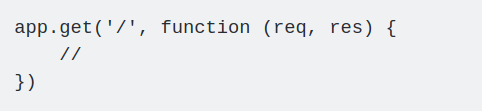
\includegraphics[width = 10cm]{image/res-req.png}
        \caption{Request \& Response}
        \label{fig:req_res}
    \end{figure}
    \begin{itemize}
        \item \textbf{Request} - Biểu diễn một HTTP request và có các thuộc tính cho các request như các chuỗi truy vấn, tham số, body, HTTP header và những phần khác.
        \item \textbf{Response} - Biểu diễn một HTTP response được ứng dụng Express gửi đi khi nó nhận về một HTTP request.
    \end{itemize}
    \item \textbf{Express route}\\
    Route là một thành phần cực kỳ quan trọng của một website, nó giúp website biết được người dùng truy cập đến nơi nào của trang web, từ đó phản hồi lại một cách thích hợp. Trong ExpressJs, route được tích hợp sẵn và dễ dàng sử dụng.
    \begin{enumerate}
        \item \textbf{Route methods}
        \begin{itemize}
            \item Có 4 phương thức \textbf{GET, POST, PUT, DELETE}
            \item Ví dụ về cách sử dụng: app.get('/', (req, res) => res.send('Hello World!'));
        \end{itemize}
        \item \textbf{Route parameters}
        \begin{figure}[H]
        \centering
        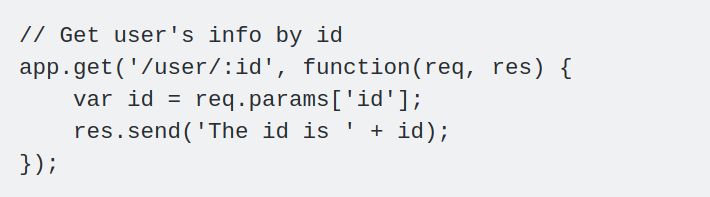
\includegraphics[width = 10cm]{image/route-parameter.png}
        \caption{Ví dụ về Route Parameter}
        \label{fig:route_parameter}
    \end{figure}
    \end{enumerate}
\end{enumerate}

\newpage
\section{Cơ sở dữ liệu}
\textbf{Khái niệm:}

Cơ sở dữ liệu (Database) là một tập hợp các dữ liệu có tổ chức, thường được lưu trữ và truy cập điện tử từ hệ thống máy tính. Khi cơ sở dữ liệu phức tạp hơn, chúng thường được phát triển bằng cách sử dụng các kỹ thuật thiết kế và mô hình hóa chính thức.\\

\textbf{Phân loại:}
\begin{itemize}
    \item Cơ sở dữ liệu quan hệ (SQL)
    \item Cơ sở dữ liệu phi quan hệ (NoSQL)
\end{itemize}

\textbf{So sánh cơ sở dữ liệu quan hệ và phi quan hệ:}
\begin{table}[H]
	    \centering
	    \begin{tabular}{|p{3cm}|p{6cm}|p{6cm}|}
	    \hline
	    &Cơ sở dữ liệu quan hệ&Cơ sở dữ liệu phi quan hệ\\
	    \hline
	    Ngôn ngữ truy vấn&Ngữ truy vấn có cấu trúc&Sử dụng ngôn ngữ truy vấn không cấu trúc\\
	    \hline
	    Cấu trúc&Biểu thị dữ liệu dưới dạng bảng, hàng và cột&Biểu thị dữ liệu dưới dạng biểu đồ, các cặp khóa-giá trị và nhiều hơn thế.\\
	    \hline
	    Khả năng mở rộng&Mở rộng thêm chiều dọc&Mở rộng theo chiều ngang\\
	    \hline
	    Chi phí&Chi phí xây dựng và bảo trì cao&Khoảng 10\% so với cơ sở dữ liệu quan hệ\\
	    \hline
	    \end{tabular}
	    \caption{So sánh cơ sở dữ liệu quan hệ và phi quan hệ}
\end{table}
\subsection{Ngôn ngữ truy vấn có cấu trúc (SQL)}
\subsubsection{SQL là gì?}
SQL là loại ngôn ngữ máy tính, giúp cho thao tác lưu trữ và truy xuất dữ liệu được lưu trữ trong một cơ sở dữ liệu quan hệ. SQL là viết tắt của Structured Query Language là ngôn ngữ truy vấn có cấu trúc.

Tất cả RDBMS (hệ thống quản lý cơ sở dữ liệu quan hệ) như đều sử dụng SQL như là ngôn ngữ cơ sở dữ liệu chuẩn.

SQL là một ngôn ngữ được tiêu chuẩn hóa bởi ANSI (American National Standards Institute) – Viện tiêu chuẩn quốc gia Hoa Kỳ. Đây cũng đồng thời là ngôn ngữ được sử dụng phổ biến trong các hệ thống quản lý cơ sở dữ liệu quan hệ và hỗ trợ sử dụng trong các công ty lớn về công nghệ.
\subsubsection{Tại sao phải sử dụng SQL?}
SQL thường được các RDBMS sử dụng để tương tác với cơ sở dữ liệu thông qua các thao tác sau:
\begin{itemize}
    \item Tạo cơ sở dữ liệu, bảng và view mới.
    \item Để chèn các bản ghi vào trong một cơ sở dữ liệu.
    \item Để xóa các bản ghi từ một cơ sở dữ liệu.
    \item Để lấy dữ liệu từ một cơ sở dữ liệu.
\end{itemize}
\subsubsection{Chức năng}
Một trong những lý do khiến cho SQL được sử dụng phổ biến, chính là nó đã cho phép người dùng thực hiện đa dạng các chức năng sau:
\begin{itemize}
    \item Cho phép người dùng truy cập dữ liệu trong các hệ thống quản lý cơ sở dữ liệu quan hệ.
    \item Cho phép người dùng mô tả dữ liệu.
    \item Cho phép người dùng xác định dữ liệu trong cơ sở dữ liệu và thao tác dữ liệu đó.
    \item Cho phép nhúng trong các ngôn ngữ khác sử dụng mô-đun SQL, thư viện và trình biên dịch trước.
    \item Cho phép người dùng tạo và thả các cơ sở dữ liệu và bảng.
    \item Cho phép người dùng tạo chế độ view, thủ tục lưu trữ, chức năng trong cơ sở dữ liệu.
    \item Cho phép người dùng thiết lập quyền trên các bảng, thủ tục và view.
\end{itemize}
\subsubsection{Ưu điểm}
\begin{itemize}
    \item Dữ liệu có ở mọi nơi: Dữ liệu xuất hiện ở mọi nơi trên màn hình từ laptop đến điện thoại của bạn. Việc học tập và tìm hiểu SQL sẽ giúp bạn biết được cách thức hoạt động của những dữ liệu này.
    \item Thêm, sửa, đọc và xóa dữ liệu dễ dàng: với SQL, các thao tác xử lý dữ liệu trở nên dễ dàng hơn bao giờ hết. Bạn chỉ cần thực hiện một số thao tác với dữ liệu đơn giản trên SQL thay vì phải dùng nhiều câu lệnh phức tạp trên các loại ngôn ngữ khác.
    \item SQL giúp công việc lập trình dễ dàng hơn: bạn có thể lưu nhiều dữ liệu cho nhiều ứng dụng khác nhau trên cũng một cơ sở dữ liệu và việc truy cập các cơ sở dữ liệu này trở lên đơn giản hơn nhờ một cách thức giống nhau.
    \item Được sử dụng và hỗ trợ bởi nhiều công ty lớn: tất cả các công ty lớn về công nghệ trên thế giới hiện nay như Microsoft, IBM, Oracle… đều hỗ trợ việc phát triển ngôn ngữ SQL.
    \item Lịch sử hơn 40 năm: với lịch sử phát triển hơn 40 năm từ 1970, SQL vẫn tồn tại và trụ vững đến ngày nay. Điều này cho thấy vị trí của SQL hiện tại rất khó bị thay thế bởi bất kỳ một ngôn ngữ máy tính nào khác.
\end{itemize}
\subsection{Hệ cơ sở dữ liệu quan hệ (RDBMS)}
\textbf{Khái niệm:}

RDBMS - Relational Database Management System - là hệ cơ sở dữ liệu quan hệ. Tất cả các hệ thống quản trị cơ sở dữ liệu hiện đại như SQL, MySQL, MS SQL Server, Oracle, ... đều dựa trên RDBMS.

Hệ thống quản lý cơ sở dữ liệu quan hệ (RDBMS) là một hệ thống quản lý cơ sở dữ liệu (DBMS) dựa trên mô hình quan hệ được giới thiệu bởi EF Codd.\\

\textbf{Bảng (Table):}

RDBMS sử dụng các bảng để lưu trữ dữ liệu. Mỗi bảng là một tập hợp các dữ liệu có liên quan đến nhau và có nhiều hàng và cột để lưu dữ liệu. Bảng là hình thức lưu trữ phổ biến và đơn giản nhất trong môt cơ sở dữ liệu quan hệ. Ví dụ về bảng một nhóm môn học trong bảng MONHOC sau đây:\\
\begin{table}[H]
    \centering
    \begin{tabular}{|l|l|l|}
    \hline
         \textbf{ID}&\textbf{TEN\_MON\_HOC}&\textbf{SO\_TIN\_CHI}\\
         \hline
         1&Giải tích 1&4\\
		\hline
		2&Vật lý&3\\
		\hline			
		3&Kỹ thuật lập trình&4\\
		\hline
    \end{tabular}
    \caption{Ví dụ về bảng dữ liệu}
\end{table}

\textbf{Trường (Field):}
	
	Mỗi bảng được chia thành các thực thể nhỏ gọi là các trường, chứa các thông tin cụ thể về mỗi bản ghi trong bảng. Các trường trong bảng MONHOC bao gồm: ID, TEN\_MON\_HOC, SO\_TIN\_CHI.\\
	\begin{table}[H]
	    \centering
	    \begin{tabular}{|l|}
	        \hline
	        \textbf{TEN\_MON\_HOC}\\
	        \hline
	        Giải tích 1\\
	        \hline
	        Vật lý\\
	        \hline
	        Kỹ thuật lập trình\\
	        \hline
	    \end{tabular}
	    \caption{Ví dụ một trường trong bảng dữ liệu}
	\end{table}
	
\textbf{Hàng hoặc bản ghi (Record):}
	
Một hàng của bảng được gọi là bản ghi , nó chứa thông tin của một đối tượng trong bảng. Ví dụ ở bảng MONHOC có 3 bản ghi. Sau đây là một bản ghi trong bảng:\\
\begin{table}[H]
    \centering
    \begin{tabular}{|r|r|r|}
        \hline
		1&Giải tích 1&4\\
		\hline
    \end{tabular}
    \caption{Ví dụ về một bản ghi}
\end{table}
\newpage
\textbf{Ràng buộc (Constraint):}

Ràng buộc là các quy tắc cho các cột dữ liệu trong bảng. Chúng được sử dụng để giới hạn loại dữ liệu có thể insert vào một bảng. Điều này đảm bảo tính chính xác và độ tin cậy của dữ liệu trong cơ sở dữ liệu.\\
Constraint có thể là cấp độ cột hoặc cấp độ bảng. Các ràng buộc cấp độ cột chỉ được áp dụng cho một
cột trong khi các ràng buộc mức bảng được áp dụng cho toàn bộ bảng.\\
Sau đây là một số ràng buộc phổ biến nhất được sử dụng trong SQL :\\
\begin{table}[H]
    \centering
    \begin{tabular}{|l|l|}
        \hline
         NOT NULL&Đảm bảo rằng một field không có giá trị NULL  \\
         \hline
         DEFAULT&Cung cấp giá trị mặc định của một field khi không được xác định\\
         \hline
         UNIQUE&Đảm bảo giá trị trong một field là khác nhau\\
         \hline
         PRIMARY Key&Mỗi record là duy nhất trong một bảng cơ sở dữ liệu\\
         \hline
         FOREIGN Key&Mỗi record là duy nhất trong trong bất kỳ bảng cơ sở dữ liệu khác\\
         \hline
         CHECK&Đảm bảo rằng tất cả các giá trị trong một cột thỏa mãm một số điều kiện\\
         \hline
         INDEX&Dùng để tạo và lấy dữ liệu một cách nhanh chóng\\
         \hline
    \end{tabular}
    \caption{Một số ràng buộc phổ biến trong SQL}
\end{table}
\subsection{Hệ quản trị cơ sở dữ liệu}

Hệ quản trị cơ sở dữ liệu (Database Management System - DBMS) là hệ thống kiểm soát việc lưu trữ, tổ chức và truy xuất dữ liệu.

Mỗi DBMS đều có thành phần gọi là Query Language (Ngôn ngữ truy vấn), các ứng dụng muốn truy cập dữ liệu đều phải nhờ vào thành phần này.

Các hệ quản trị cơ sở dữ liệu quan hệ phổ biến nhất hiện nay:
\subsubsection{Oracle Database}
\begin{center}
  \captionsetup{type=figure}
  
\includegraphics[scale=0.4]{image/oracle.jpg}
  \captionof{figure}{Oracle Database}
\end{center}


\textbf{Oracle là gì?}


Oracle Database hay còn gọi là Oracle RDBMS hoặc đơn giản là Oracle là 1 hệ quản trị cơ sở dữ liệu quan hệ, được phát triển và phân phối bởi tập đoàn Oracle

Cơ sở dữ liệu Oracle là cơ sở dữ liệu đầu tiên được thiết kế cho điện toán lưới doanh nghiệp, cách linh hoạt và tiết kiệm chi phí nhất để quản lý thông tin và ứng dụng. Điện toán lưới doanh nghiệp tạo ra các nhóm lớn máy chủ và lưu trữ mô-đun theo tiêu chuẩn công nghiệp. Với kiến trúc này, mỗi hệ thống mới có thể được cung cấp nhanh chóng từ nhóm các thành phần. Không cần khối lượng công việc cao nhất, bởi vì công suất có thể dễ dàng được thêm hoặc phân bổ lại từ các nguồn tài nguyên khi cần thiết.\\

\textbf{Đặc điểm của Oracle}
\begin{itemize}
    \item Quản lý được hệ thống dữ liệu lớn
    \item Hỗ trợ nhiều công cụ để quản trị cũng như nhập, xuất dữ liệu dễ dàng
    \item Có thể hoạt động trên nhiều hệ điều hành khác nhau như Windows, Linux, Mac OS, Unix,...
    \item Truy cập đồng thời
    \item Hỗ trợ cơ chế khóa
    \item Thực thi song song
    \item Tính khả chuyển
\end{itemize}

\textbf{Thế mạnh của Oracle:}
\begin{itemize}
    \item \textit{Hệ thống quản lý và kiểm soát tập trung:} Điều này cho phép dữ liệu được kiểm soát hoàn toàn từ một trao đổi dạng bảng vì nó chịu trách nhiệm gán, thêm, xóa các bản ghi và sửa đổi chúng.
    \item \textit{Tiêu chuẩn hóa:} Cho phép tiêu chuẩn hóa giữa các triển khai SQL khác nhau.
    \item \textit{Nhóm các giao dịch:} Nó cho phép nhóm một số giao dịch và chia từng hoạt động thành các phân khúc và do đó đạt được hiệu suất tốt hơn trong thời gian ngắn hơn có thể.
    \item \textit{Phương thức hiệu suất:} Áp dụng các phương pháp để cải thiện cơ sở dữ liệu thông qua ứng dụng Cluster.
\end{itemize}
\subsubsection{MySQL}
\begin{center}
  \captionsetup{type=figure}
    
\includegraphics[scale=0.5]{image/mysql.jpg}
  \captionof{figure}{MySQL}
\end{center}

MySQL là một hệ quản trị cơ sở dữ liệu quan hệ mã nguồn mở, được phát triển, phân phối và hỗ trợ bởi tập đoàn Oracle.\\

\textbf{MySQL hoạt động như thế nào?}

MySQL hoạt động dưới hình thức client-server:
\begin{itemize}
    \item MySQL tạo một cơ sở dữ liệu để lưu trữ và thao tác dữ liệu, xác định mối quan hệ của từng bảng.
    \item Khách hàng có thể thực hiện các yêu cầu bằng cách nhập các câu lệnh SQL cụ thể trên MySQL.
    \item Ứng dụng máy chủ sẽ phản hồi với thông tin được yêu cầu và nó sẽ xuất hiện ở phía máy khách.
\end{itemize}


\textbf{Đặc điểm và thế mạnh:}
\begin{itemize}
    \item \textit{Tính nội bộ và linh động:}
    \begin{itemize}
    \item Viết bằng C và C++
    \item Đã thử nghiệm với một loạt các trình biên dịch khác nhau
    \item Hoạt động trên nhiều nền tảng khác nhau
    \item Sử dụng thiết kế máy chủ nhiều lớp với các mo-đun độc lập
    \item Được thiết kế để đa luồng hoàn toàn bằng cách sử dụng các luồng nhân, để dễ dàng sử dụng nhiều CPU nếu chúng có sẵn
    \item Triển khai các bảng băm trong bộ nhớ, được sử dụng làm bảng tạm thời.
    \item Triển khai các hàm SQL bằng cách sử dụng thư viện lớp được tối ưu hóa cao nhất phải nhanh nhất có thể
    \end{itemize}
    \item \textit{Bảo mật}
    \begin{itemize}
        \item Một hệ thống đặc quyền và mật khẩu rất linh hoạt và an toàn, và cho phép xác minh dựa trên máy chủ
        \item Bảo mật mật khẩu bằng cách mã hóa tất cả lưu lượng mật khẩu khi bạn kết nối với máy chủ.
    \end{itemize}
    \item \textit{Khả năng mở rộng và giới hạn:}
    \begin{itemize}
        \item Hỗ trợ cơ sở dữ liệu lớn
        \item Hỗ trợ lên đến 64 chỉ mục cho mỗi bảng
    \end{itemize}
    \item \textit{Ổn định, có tốc độ cao và dễ sử dụng}
    \item \textit{Đa tính năng:} Hỗ trợ rất nhiều chức năng SQL
\end{itemize}
\subsubsection{SQL Server}
\begin{center}
  \captionsetup{type=figure}
    
\includegraphics[scale=0.3]{image/sql-server.png}
  \captionof{figure}{SQL Server}
\end{center}
\textbf{SQL Server là gì?}

SQL Server là một RDBMS được phát triển bởi tập đoàn Microsoft. Tương tự như phần mềm RDBMS khác, SQL Server được xây dựng dựa trên SQL, một ngôn ngữ lập trình tiêu chuẩn để tương tác với các cơ sở dữ liệu quan hệ. Máy chủ SQL được liên kết với Transact-SQL hoặc T-SQL, triển khai SQL Microsoft Microsoft bổ sung một tập hợp các cấu trúc lập trình độc quyền. SQL Server hoạt động độc quyền trên môi trường Windows trong hơn 20 năm. Năm 2016, Microsoft đã cung cấp nó trên Linux. SQL Server 2017 thường có sẵn vào tháng 10 năm 2016 chạy trên cả Windows và Linux.\\
\newline
\textbf{SQL Server hoạt động như thế nào?}
\begin{itemize}
    \item Giống như các công nghệ RDBMS khác, SQL Server chủ yếu được xây dựng xung quanh cấu trúc bảng dựa trên hàng để kết nối các thành phần dữ liệu liên quan trong các bảng khác nhau với nhau, tránh việc lưu trữ dữ liệu ở nhiều nơi trong cơ sở dữ liệu. Mô hình quan hệ cũng cung cấp tính toàn vẹn tham chiếu và các ràng buộc toàn vẹn khác để duy trì độ chính xác của dữ liệu. Các kiểm tra này là một phần của việc tuân thủ rộng hơn các nguyên tắc về tính nguyên tử, tính nhất quán, độ cô lập và độ bền, được gọi chung là các thuộc tính ACID và được thiết kế để đảm bảo rằng các giao dịch cơ sở dữ liệu được xử lý một cách đáng tin cậy.
    \item Thành phần cốt lõi của SQL Server là SQL Server Database Engine, điều khiển lưu trữ, xử lý và bảo mật dữ liệu. Nó bao gồm một công cụ quan hệ xử lý các lệnh và truy vấn và một công cụ lưu trữ quản lý các tệp cơ sở dữ liệu, bảng, trang, chỉ mục, bộ đệm dữ liệu và giao dịch. Các thủ tục lưu trữ, kích hoạt, khung nhìn và các đối tượng cơ sở dữ liệu khác cũng được tạo bởi Cơ sở dữ liệu.
    \item Bên dưới cơ sở dữ liệu là Hệ điều hành Máy chủ SQL hoặc SQLOS. SQLOS xử lý các chức năng cấp thấp hơn, chẳng hạn như quản lý bộ nhớ và I/O, lập lịch công việc và khóa dữ liệu để tránh các cập nhật xung đột. Một lớp giao diện mạng nằm phía trên Cơ sở dữ liệu và sử dụng giao thức Luồng dữ liệu dạng bảng của Microsoft để tạo điều kiện cho các tương tác yêu cầu và phản hồi với các máy chủ cơ sở dữ liệu. Và ở cấp độ người dùng, các DBA và nhà phát triển SQL Server viết các câu lệnh T-SQL để xây dựng và sửa đổi cấu trúc cơ sở dữ liệu, thao tác dữ liệu, thực hiện bảo vệ an ninh và sao lưu cơ sở dữ liệu, trong số các tác vụ khác
\end{itemize}
\textbf{Thế mạnh:}
\begin{itemize}
    \item Cho phép nhiều người dùng chung một cơ sở dữ liệu
    \item Duy trì lưu trữ bền vững
    \item Khả năng mở rộng
    \item Tính bảo mật cao
    \item Độ tin cậy, bảo vệ dữ liệu
    \item Hỗ trợ phân tích dữ liệu
    \item Kết hợp tốt với các sản phẩm của Microsoft
    \item Có thể sao lưu, khôi phục dữ liệu một cách dễ dàng
\end{itemize}

\subsubsection{PostgreSQL}
\begin{center}
  \captionsetup{type=figure}
    
\includegraphics[scale=0.5]{image/postgre-sql.jpg}
  \captionof{figure}{PostgreSQL}
\end{center}

PostgreSQL là một RDBMS mở nguồn mở được xây dựng trên mã nguồn ban đầu của đại học Berkeley.

\textit{Đặc điểm và thế mạnh:}
\begin{itemize}
    \item Truy xuất dữ liệu tốc độ nhanh
    \item Sử dụng câu truy vấn phức tạp
    \item Sử dụng khóa ngoại
    \item Có thủ tục
    \item Đảm bảo tính toàn vẹn của các giao tác
\end{itemize}

\subsection{Hệ cơ sở dữ liệu phi quan hệ (Non-RDBMS)}
Hệ cơ sở dữ liệu phi quan hệ là cơ sở dữ liệu không sử dụng mô hình bảng gồm các cột và hàng như nhiều hệ cơ sở dữ liệu truyền thống. Thay vào đó, Non-RDBMS sử dụng mô hình lưu trữ được tối ưu hóa cho các yêu cầu cụ thể của loại dữ liệu được lưu trữ. Cơ sở dữ liệu phi quan hệ (Non-relational database) phổ biến nhất được gọi là NoSQL.\\
Các Non-RDBMS phổ biến:
\subsubsection{MongoDB}
\begin{center}
  \captionsetup{type=figure}
    
\includegraphics[width=10cm]{image/mongo.png}
  \captionof{figure}{MongoDB}
\end{center}

MongoDB (chữ mongo được lấy từ từ humongous trong tiếng Anh), là một NoSQL database. Khác với MySQL hay các loại SQL databse khác chạy theo mô hình database – table – row với số dòng – cột nhất định, schema phức tạp, và phải sử dụng nhiều Join khi query. MongoDB chạy theo mô hình database – collection – document, thay thế mô hình cơ sở dữ liệu dùng table truyền thống bằng các document với định dạng JSON với cấu trúc linh hoạt hơn (MongoDB gọi là BSON).

Các thuật ngữ thường sử dụng trong MongoDB:
\begin{itemize}
    \item \textbf{\_id:} Là trường bắt buộc có trong mỗi document. Trường \_id đại diện cho một giá trị duy nhất trong document MongoDB. Trường \_id cũng có thể được hiểu là khóa chính trong document. Nếu bạn thêm mới một document thì MongoDB sẽ tự động sinh ra một \_id.
    \item \textbf{Collection:} Collection là một nhóm các Document trong MongoDB. Nó tương đương như một bảng trong RDBMS. Do đó, một Collection tồn tại bên trong một cơ sở dữ liệu duy nhất. Các Collection không có ràng buộc Relationship như các hệ quản trị cơ sở dữ liệu khác nên việc truy xuất rất nhanh, chính vì thế mỗi collection có thể chứa nhiều thể loại khác nhau không giống như table trong hệ quản trị mysql là các field cố định. Các Document bên trong một Collection có thể có nhiều trường khác nhau. Đặc biệt, tất cả các Document trong một Collection là tương tự nhau hoặc với cùng mục đích liên quan.
    \item \textbf{Cursor:} Đây là một con trỏ đến tập kết quả của một truy vấn. Máy khách có thể lặp qua một con trỏ để lấy kết quả.
    \item \textbf{Database:} Chính là tập chứa các collection trong MongoDB. Mỗi database sẽ có một tập file riêng của mình trên file system của hệ thống. Một MongoDB server thường chứa nhiều database trên đó.
    \item \textbf{Document:} Là một tập dữ liệu theo dạng key-value, mỗi key sẽ tương ứng với một value. Các document khá linh hoạt về schema, như đã nói ở trên, các document trong cùng một collection không nhất thiết phải có các field hoặc cấu trúc giống nhau. Data trong cùng một field cũng có thể có nhiều kiểu dữ liệu khác nhau.
    \item \textbf{Field:} Là một cặp name-value trong một document.
    \item \textbf{JSON:} Các document của MongoDB sử dụng format JSON (JavaScript Object Notation), đây là một chuẩn lưu trữ, trao đổi dữ liệu đơn giản và gọn nhẹ. Với ưu điểm dễ đọc, dễ hiểu, đa phần các ngôn ngữ lập trình phổ biến hiện nay đều hỗ trợ JSON như: C, C++, Java, JavaScript, Perl, Python,….Dữ liêu trong JSON được lưu trữ dưới dạng key/value. Một key sẽ tương ứng với 1 value. Value ở đây có thể là một mảng, một chuỗi, một số int, double, mảng hoặc object… .
    
    
\end{itemize}

\textit{Thế mạnh:}
\begin{itemize}
    \item Ít schema hơn
    \item Cấu trúc của một đối tượng rõ ràng
    \item Không có các phép join phức tạp
    \item Khả năng mở rộng cực lớn: Việc mở rộng dữ liệu mà không cần phải quan tâm đến các vấn đề như khóa ngoại, khóa chính, kiểm tra ràng buộc,...
    \item Sử dụng bộ nhớ trong để lưu giữ cửa sổ làm việc cho phép truy cập dữ liệu nhanh hơn. Việc cập nhật được thực hiện nhanh gọn nhờ update tại chỗ (in-place).
    \item Hỗ trợ nhiều công cụ lưu trữ
\end{itemize}

\textit{Các thao tác cơ bản trong MongoDB}
\begin{description}
\item 1.Create:\\
Tạo hoặc thêm một document mới vào collection, nếu collection đó chưa tồn tại thì sẽ tạo mới collection

MongoDB cung cấp hai phương thức để chèn thêm một document:
\begin{itemize}
    \item db.collection.insertOne(): chèn một tài liệu mới vào một collection. Nếu document không có trường \_id , MongoDB sẽ tự động thêm trường \_id với value kiểu ObjectId.
\begin{verbatim}
db.inventory.insertOne(
    { item: "canvas", qty: 100, tags: ["cotton"], size:{ h: 28, w: 35.5}}
)
\end{verbatim}
    \item db.collection.insertMany(): chèn nhiều document vào một collection, truyền vào phương thức là mảng các document
\begin{verbatim}
db.inventory.insertMany([
    {item: "journal", qty: 25, tags: ["blank", "red"], size:{h: 14, w: 21}},
    {item: "mat", qty: 85, tags: ["gray"], size:{h: 27.9, w: 35.5}},
    {item: "mouse", qty: 25, tags: ["gel", "blue"], size:{h: 19, w: 22.85}}
])
\end{verbatim}
\end{itemize}
\item 2.Read\\
Truy xuất document từ một collection. Để lấy ra toàn bộ document của ta sử dụng phương thức find
\begin{verbatim}
        db.inventory.find()
\end{verbatim}
\item 3. Update\\
Thao tác update cho phép chình sửa document trong collection
\begin{itemize}
    \item Cập nhật một document với db.collection.updateOne():
    \begin{verbatim}
        db.inventory.updateOne(
           { item: "paper" },
           {
             $set: { "size.uom": "cm", status: "P" }
           }
        )
    \end{verbatim}
    \item Cập nhật nhiều Document với db.collection.updateMany():
    \begin{verbatim}
        db.inventory.updateMany(
           { "qty": { $lt: 50 } },
           {
             $set: { "size.uom": "in", status: "P" },
             $currentDate: { lastModified: true }
           }
        )
    \end{verbatim}
    \item Thay thế một document: Để thay thế toàn bộ nội dung của một document (ngoại trừ trường \_id), truyền vào toàn bộ document mới là một tham số thứ hai của hàm. Ví dụ dưới đây thay thế document đầu tiên từ collection inventory mà có item bằng "paper"
\begin{verbatim}
db.inventory.replaceOne(
    {item:"paper"},
    {item: "paper",instock:[{warehouse:"A",qty:60},{warehouse:"B",qty:40}]}
)
\end{verbatim}
\end{itemize}
\item 4. Delete\\
\begin{itemize}
    \item Xóa một document thỏa mãn điều kiện: Để xóa chỉ một document phù hợp với điều kiện (trường hợp có nhiều document thỏa mãn thì sẽ xóa document đầu tiên), sử dụng db.collection.deleteOne(filter)
    \item Xóa tất cả document thỏa mãn điều kiện: sử dụng db.collection.deleteMany(filter)

\end{itemize}
\end{description}
\subsection{So sánh Relational Database và Non-Relational Database}
\begin{table}[H]
	    \centering
	    \begin{tabular}{|p{3cm}|p{6cm}|p{6cm}|}
	        \hline
	        &\textbf{Relational}&\textbf{Non-Relational}\\
	        \hline
	        Ngôn ngữ truy vấn&Ngôn ngữ truy vấn có cấu trúc &Truy vấn đối tượng: trực quan, chuyển một tài liệu để giải thích những gì bạn đang truy vấn\\
	        \hline
	        Kiểu dữ liệu&Lưu các kiểu dữ liệu được quy định&Có thể lưu bất kỳ loại dữ liệu nào\\
	        \hline
	        Khả năng mở rộng&Mở rộng thêm chiều dọc&Mở rộng theo chiều ngang\\
	        \hline
	        Hiển thị dữ liệu&Dưới dạng bảng và hàng&Dưới dạng JSON\\
	        \hline
	        Chi phí&Chi phí xây dựng và bảo trì cao&Khoảng 10\% so với Relational\\
	        \hline
	    \end{tabular}
	    \caption{So sánh cơ sở dữ liệu quan hệ và cơ sở dữ liệu phi quan hệ}
	\end{table}
\subsection{Kết luận và lựa chọn}

Dựa vào các đối tượng mà hệ thống hướng tới, hệ thống cần lưu trữ lượng dữ liệu lớn, đáp ứng trong thời gian nhanh. Nhóm quyết định lựa chọn sửa dụng \textbf{MongoDB}.\\
\begin{itemize}
    \item Dữ liệu trong MongoDB không có sự ràng buộc lẫn nhau như trong RDBMS, khi insert, xóa hay update nó không cần phải mất thời gian kiểm tra xem có thỏa mãn các bảng liên quan như trong RDBMS.
    \item Dữ liệu trong MongoDB được đánh chỉ mục (đánh index) nên khi truy vấn nó sẽ tìm rất nhanh
    \item Khi thực hiện insert, find… MongoDB sẽ khóa các thao tác khác lại, ví dụ khi nó thực hiện find(), trong quá trình find mà có thêm thao tác insert, update thì nó sẽ dừng hết lại để chờ find() xong đã.

\end{itemize}


% \textbf{Node-oracledb:}
% Thay vì phải sử dụng các câu query thuần để kết nối, truy cập, định nghĩa cấu trúc
% database, chúng ta có thể sử dụng các hàm do Node-oracledb cung cấp để làm những việc này
% một cách dễ dàng, ngắn gọn, nhanh chóng hơn.
% \begin{figure}[ht]
%     \centering
%     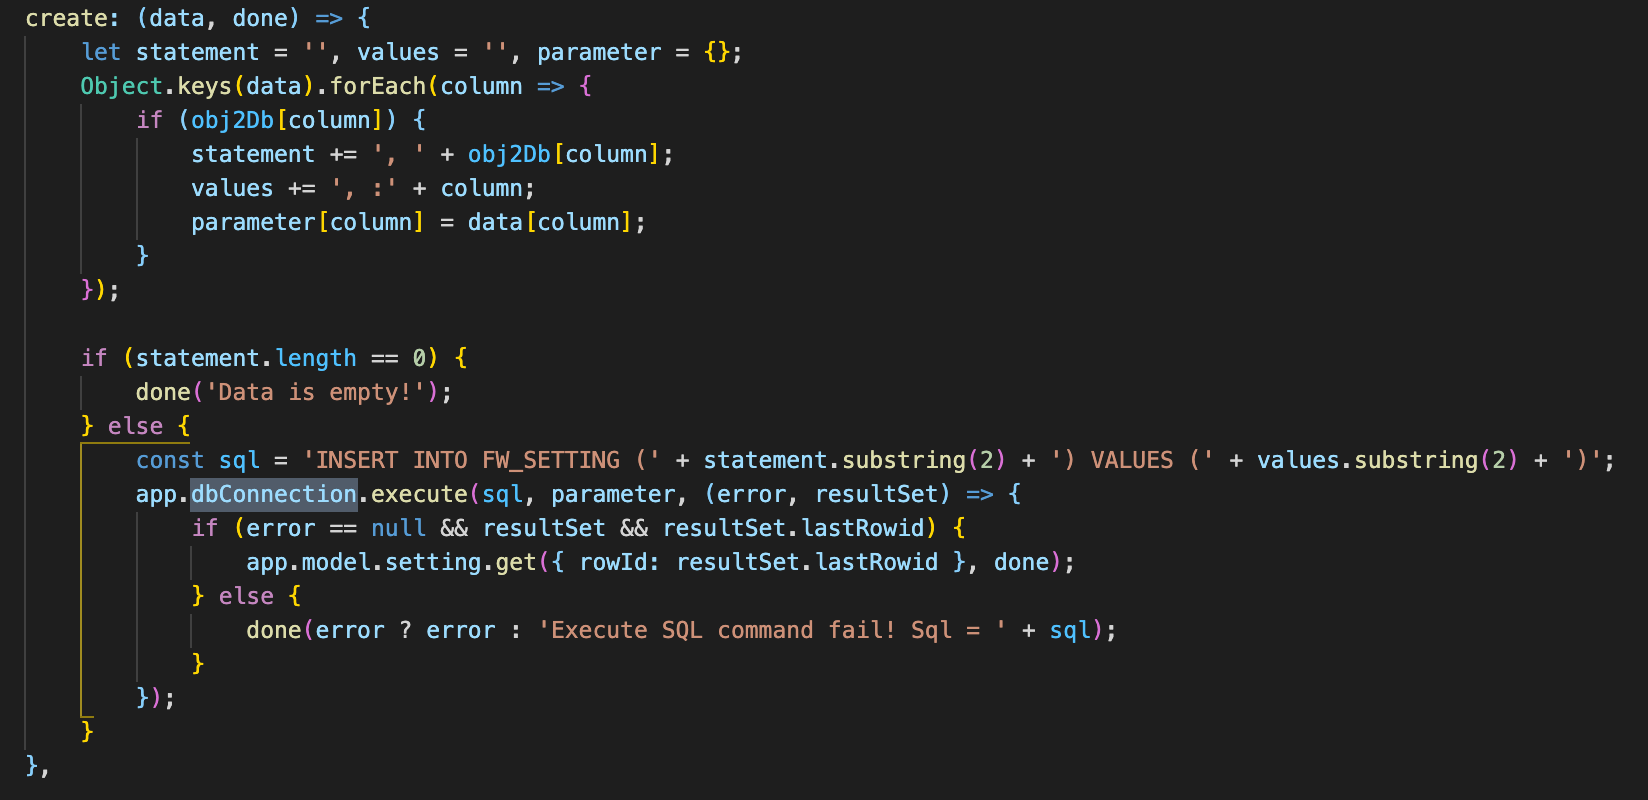
\includegraphics[width=10cm]{image/nodeoracledb.png}
%     \caption{Ví dụ về việc sử dụng node-oracledb}
% \end{figure}


% Việc truy vấn dữ liệu cũng dễ dàng, thuận tiện hơn khi Node-oracledb hỗ trợ các hàm truy
% vấn.
\section{REST API}
\subsection{Giới thiệu REST API:}
REST (REpresentational State Transfer) là một tiêu chuẩn thiết kế API (API architectural style) cho các ứng dụng. REST được giới thiệu lần đầu tiên bởi Roy Fielding vào năm 2000 trong luận án nổi tiếng của ông ``Architectural Styles and
the Design of Network-based Software Architecture'' đại học California.

Mặc dù REST có thể sử dụng trên hầu hết mọi giao thức ứng dụng phần mềm, nhưng REST thường biết đến rộng rãi trong các giao thức của ứng dụng Web vì tận dụng được những lợi thế của HTTP, giúp nhà phát triển không cần cài đặt thêm phần mềm hoặc thư viện bổ sung để sử dụng REST API.

\subsection{Một số đặc điểm cơ bản của REST:}
\begin{itemize}
    \item \textbf{Uniform interface:} Các API được thiết kế một cách nhất quán theo các nguyên tắc chung. Ví dụ luôn luôn sử dụng danh từ số nhiều thay vì khi số nhiều, khi số ít, sử dụng dấu gạch ngang để phân tách giữa các từ. Tài nguyên của hệ thống phải tuân theo các quy tắt đặt tên, định dạng dữ liệu (JSON hay XML), được truy cập thông qua một cách tiếp cận phổ biến như HTTP GET và được sửa đổi thông qua các phương thức tương tự.
    \item \textbf{Client-Server:} Client và Server không cần phụ thuộc vào nhau, có thể phát triển độc lập, thậm chí sửa đổi, thay thế miễn sao interface giao tiếp giữa chúng vẫn được giữ nguyên.
    \item \textbf{Stateless}: Server không lưu trữ bất kì thông tin gì về yêu cầu của client, nó sẽ coi mọi yêu cầu là mới. Không section, không history. Vì vậy, mỗi yêu cầu từ client tới server phải chứa tất cả các thông tin cần thiết để  server hiểu được yêu cầu đó.
    \item \textbf{Code on demand:} Sử dụng HTTP status code khi có thể
\end{itemize}


\subsection{Những lợi ích khi sử dụng REST API:}

- Nhờ tính độc lập giữa client và server, nhà phát triển có thể dễ dàng phát triển, sửa đổi thậm chí thay thế client và server miễn sao vẫn giữ nguyên interface giao tiếp giữa chúng.

- API REST luôn độc lập với loại nền tảng hoặc ngôn ngữ: API REST luôn thích nghi với loại cú pháp hoặc nền tảng đang được sử dụng, điều này mang lại sự tự do đáng kể khi thay đổi hoặc kiểm tra môi trường mới trong quá trình phát triển. Với API REST, bạn có thể có máy chủ với các ngôn ngữ như PHP, Java, Python hoặc Node.js.

- Tính nhất quán: Các API được thiết kế một cách nhất quán giúp cho việc phát triển, bảo trì đơn giản hơn, đặc biệt phù hợp với các hệ thống có nhiều module.